\begin{figure}[t]
\begin{center}
\begin{small}
\begin{sc}
\begin{subfigure}[b]{.49\textwidth}
\begin{center}
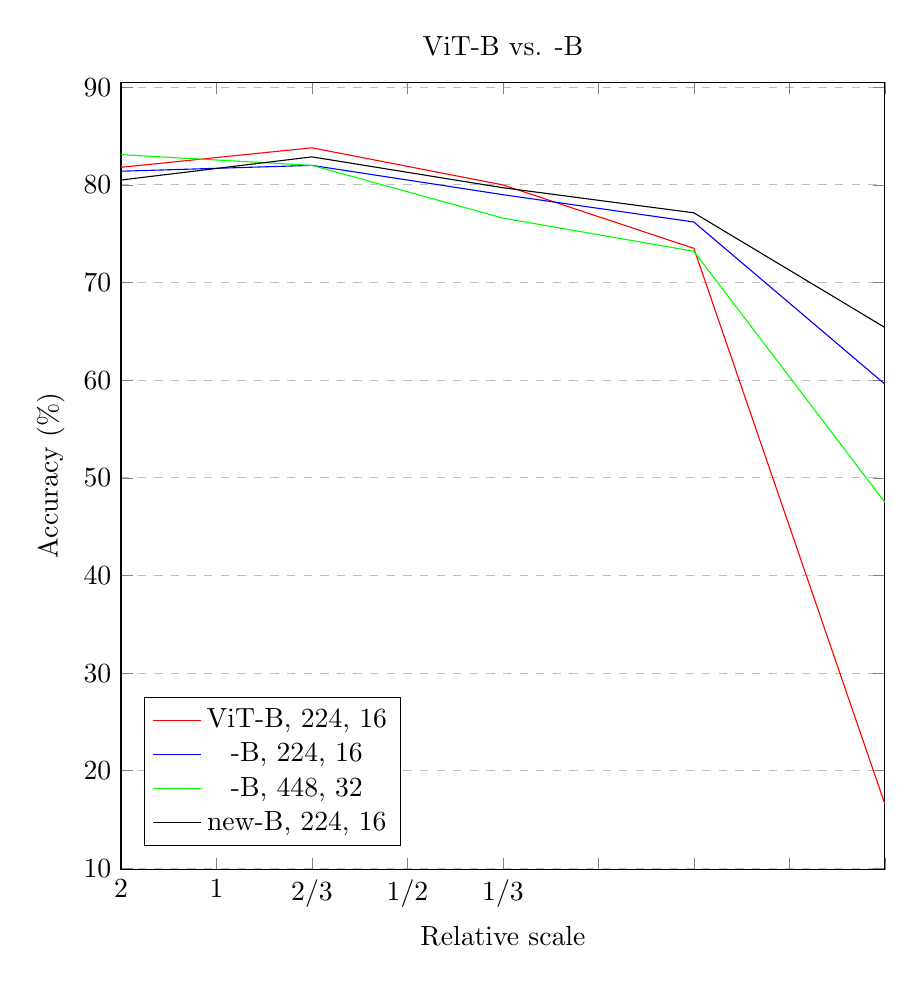
\begin{tikzpicture}
\begin{axis}[
    title={ViT-B vs. \ours{}-B},
    xlabel={Relative scale},
    ylabel={Accuracy (\%)},
    xticklabels={0,2,1,$2/3$,$1/2$,$1/3$},
    xmin=1,
    xmax=5,
    ymajorgrids=true,
    grid style=dashed,
    scale only axis,
    height=10cm,
    width=.8\linewidth,
    legend pos=south west
]
    \addplot[color=red]
    coordinates {
    (1,81.8)(2,83.8)(3,80.0)(4,73.5)(5,16.6)
    };
    \addlegendentry{ViT-B, 224, 16}
    \addplot[color=blue]
    coordinates {
    (1,81.4)(2,82.0)(3,79.0)(4,76.2)(5,59.6)
    };
    \addlegendentry{\ours{}-B, 224, 16}
    \addplot[color=green]
    coordinates {
    (1,83.1)(2,82.0)(3,76.6)(4,73.2)(5,47.5)
    };
    \addlegendentry{\ours{}-B, 448, 32}
    \addplot[color=black]
    coordinates {
    (1,80.5)(2,82.87)(3,79.71)(4,77.14)(5,65.4)
    };
    \addlegendentry{new\ours{}-B, 224, 16}
\end{axis}
\end{tikzpicture}
\end{center}
\end{subfigure}
\begin{subfigure}[b]{.49\textwidth}
\begin{center}
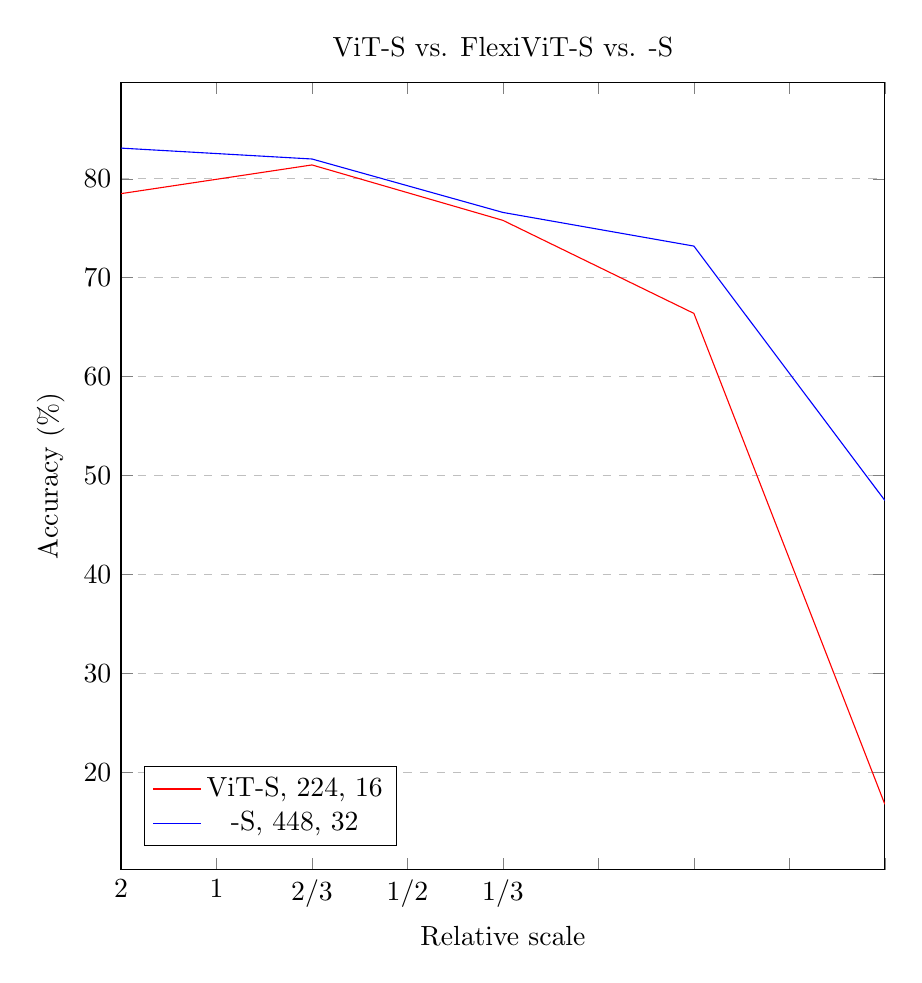
\begin{tikzpicture}
\begin{axis}[
    title={ViT-S vs. FlexiViT-S vs. \ours{}-S},
    xlabel={Relative scale},
    ylabel={Accuracy (\%)},
    xticklabels={0,2,1,$2/3$,$1/2$,$1/3$},
    xmin=1,
    xmax=5,
    ymajorgrids=true,
    grid style=dashed,
    scale only axis,
    height=10cm,
    width=.8\linewidth,
    legend pos=south west
]
    \addplot[color=red]
    coordinates {
    (1,78.5)(2,81.4)(3,75.8)(4,66.4)(5,16.8)
    };
    \addlegendentry{ViT-S, 224, 16}
    \addplot[color=blue]
    coordinates {
    (1,83.1)(2,82.0)(3,76.6)(4,73.2)(5,47.5)
    };
    \addlegendentry{\ours{}-S, 448, 32}
    
\end{axis}
\end{tikzpicture}
\end{center}
\end{subfigure}
\end{sc}
\end{small}
\end{center}

\caption{Accuracy vs. scale for grid sampling.}
\label{fig:grid-sample}
\end{figure}